\documentclass[conference]{IEEEtran}
\IEEEoverridecommandlockouts
% The preceding line is only needed to identify funding in the first footnote. If that is unneeded, please comment it out.
\usepackage{cite}
\usepackage[portuges,brazil,english]{babel}
\usepackage{amsmath,amssymb,amsfonts}
\usepackage{algorithmic}
\usepackage{graphicx}
\usepackage{textcomp}
\usepackage[export]{adjustbox}
\usepackage{float}
\usepackage[ruled,vlined,linesnumbered,portuguese]{algorithm2e}
\usepackage[utf8]{inputenc}
\def\BibTeX{{\rm B\kern-.05em{\sc i\kern-.025em b}\kern-.08em
    T\kern-.1667em\lower.7ex\hbox{E}\kern-.125emX}}
\begin{document}

\title{Trabalho 3 - MC886 Aprendizado de Máquina}

\author{\IEEEauthorblockN{Leo Yuuki Omori Omi}
\IEEEauthorblockA{
138684 \\
leoyuuki@gmail.com}
\and
\IEEEauthorblockN{João Pedro Ramos Lopes}
\IEEEauthorblockA{
139546 \\
jpedrorl@gmail.com}}

\maketitle

\section{Introdução}


Neste trabalho, temos o objetivo de explorar as técnicas de classificação vistas em aula para construir um sistema de reconhecimento de objetos para classificar imagens. Utilizando a Regressão Logística e Redes Neurais, iremos construir vários modelos para classificar imagens do conjunto de dados CIFAR-10.

\section{Regressão Logística}
 
A regressão logística é um método utilizado em Aprendizado de Máquina para classificação. Este método utiliza a função sigmóide para predizer se uma entrada é de um determinado conjunto ou não, ou seja é classificação binária.
Em casos de classificação de múltiplas classes, temos duas abordagens que foram utilizadas neste trabalho.
A abordagem Um-Contra-Todos (\textit{One-vs-All}) calcula a probabilidade estimada de cada uma das classes contra todas outras, escolhendo aquela classe que maximiza esta probabilidade.
A abordagem multinomial utiliza a função \textit{Softmax}, dando a entrada uma probabilidade para esta entrada uma probabilidade para todas as classes.

\subsection{Soluções Propostas}

\subsubsection{Solução Base (One vs All)}
A primeira solução proposta foi aplicar a regressão linear usando a classificação de múltiplas classes Um-contra-todos sobre os níveis de cinza de cada pixel da imagem (foi utilizada a função rgb2gray do Scikit-image). Foi utilizado a implementação de Regressão Logística do Scikit-learn, sendo que o parâmetro \textit{multi\_class} foi setado para \textit{ovr}.

\subsubsection{Solução Base Melhorada}
Para analisar possíveis jeitos de melhorar o modelo, foram realizados três experimentos com o objetivo de melhorar a solução base. O primeiro foi utilizar um operador de bordas nas imagens e depois realizar a regressão logística. Foi utilizado o operador de Roberts implementado no Scikit-image. O segundo exprimento foi realizar uma segmentação da imagem e aplicar a regressão logística. A segmentação foi implementada utlizando a função de Otsu para obter uma limiar para cada imagem e criar uma máscara na imagem com o intuito de isolar o objeto do plano de fundo. O terceiro experimento foi utilizar a Análise de Compenentes Principais ou \textit{Principal Component Analysis} para reduzir a dimensionalidade do modelo, utilizando a implementação do Scikit-learn.

\subsubsection{Solução Base (Multinomial)}
Esta solução utiliza a Regressão Logística Multinomial, utilizando o melhor resultado entre os experimentos anteriores (níveis de cinza, operador de bordas, segmentação ou PCA). Para esta solução utilizamos a implementação de Regressão Logística do Scikit-learn, com o parâmetro \textit{multi\_class} setado para \'multinomial\' e o parâmetro solver setado para \'sag\' (\textit{Stochastic Gradient Descent}).

\subsection{Experimentos}
\subsubsection{Modelos iniciais}
Para o modelo base e de múltiplos graus de regressão logística, utilizamos de \textit{k-fold cross-validation}, com k=5 conjuntos, para verificarmos o funcionamento dos modelos. Para os experimentos, utilizamos estes conjuntos de dados para que pudéssemos ver a acurácia (utlizando a função \textit{score} do scikit-learn) do conjunto de treino e do conjunto de validação para verificarmos se houve \textit{overfitting} (ou \textit{underfitting}). Então calculamos a média aritmética dos resultados para o conjunto de testes e validação.

\subsubsection{Solução Base (One vs All)}
A solução base que utiliza como \textit{features} os níveis de cinza de todos os pixels da imagem obteve uma acurácia para o conjunto de testes de 35\% e para o de validação 28\%. A diferença de 7\% entre a acurárcia dos dois conjuntos indica que houve um pouco de \textit{overfitting} neste caso, e além disso, obtivemos um resultado pouco satisfatório.

\subsubsection{Solução Base Melhorada}
Com o intuito de de melhorar a solução base, foram feitos experimentos utilizando funções de borda e de segmentação. A solução de função de borda trouxe resultados na média muito próximos à solução original. Poderíamos concluir à partir deste resultado, que a extração de bordas da imagem não extrai dados que sejam relevantes para a melhora do modelo, e é algo que a própria regressão logística sobre os valores de cinza da imagem original acaba considerando de certa maneira.

\begin{figure}[H]
  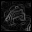
\includegraphics[center]{bor.png}
  \caption{Operador de borda}
  \label{fig:frog1}
\end{figure}

A segunda solução utilizando a segmentação obteve resultados piores de acurácia. 30\% para o conjunto de testes e 21\% no conjunto de validação. A causa desta queda pode ser atribuído à técnica simples da segmentação, já que em alguns casos a máscara pode extrair o objeto da imagem e em outros o plano de fundo, dependendo dos níveis de cinza do objeto serem maiores ou menores que o do fundo. Portanto, não obtivemos melhoras significativas com estas soluções, portanto iremos utlizar os níveis de cinza como na primeira solução proposta para as próximas soluções do trabalho.

\begin{figure}[H]
  
\includegraphics[center]{seg1.png}
  \caption{Segmentação isolando o plano de fundo}
  \label{fig:boat1}
\end{figure}

\begin{figure}[H]
  
\includegraphics[center]{seg2.png}
  \caption{Segmentação isolando o objeto}
  \label{fig:frog1}
\end{figure}

\subsubsection{Solução Base PCA}
A solução utilizando o PCA, deu resultados bons. Foi escrito um programa rodando em um laço com valores crescentes para o número de compenentes, começando com 15 componentes e aumentando em 16 em cada iteração. A execução do problema é lenta, mas nos trouxe resultados que puderam ser aproveitados. Por volta de 40 componentes, obtemos uma acurácia de 30\% tanto para o conjunto de treino como o conjunto de validação, o que foi o melhor resultado observado utilizando a regressão logística. Como obtemos uma acurácia semelhante entre os dois conjuntos, poderíamos dizer que não está ocorrendo \textit{overfitting}, diferente das soluções anteriores. Além disso, como diminuímos a dimensionalidade do modelo, obtemos uma solução computacionalmente mais leve.

\begin{table}[H]
\centering
\caption{Tabela de acurácia por número de componentes}
\label{my-label}
\begin{tabular}{lllll}
Componentes & Acurácia Treino & Acurácia Validação & & \\
15  & 0.29 & 0.29 &  &  \\
31  & 0.3  & 0.3  &  &  \\
47  & 0.3  & 0.3  &  &  \\
63  & 0.31 & 0.3  &  &  \\
79  & 0.31 & 0.3  &  &  \\
95  & 0.31 & 0.3  &  &  \\
111 & 0.31 & 0.3  &  &  \\
127 & 0.31 & 0.3  &  &  \\
143 & 0.32 & 0.3  &  &  \\
159 & 0.32 & 0.3  &  &  \\
175 & 0.32 & 0.3  &  &  \\
191 & 0.32 & 0.3  &  &  \\
207 & 0.32 & 0.3  &  &  \\
223 & 0.32 & 0.3  &  &  \\
239 & 0.32 & 0.3  &  &  \\
255 & 0.32 & 0.3  &  &  \\
271 & 0.32 & 0.29 &  &  \\
287 & 0.32 & 0.29 &  &  \\
303 & 0.32 & 0.29 &  &  \\
319 & 0.32 & 0.29 &  &  \\
335 & 0.32 & 0.29 &  &  \\
351 & 0.33 & 0.29 &  &  \\
367 & 0.33 & 0.29 &  &  \\
383 & 0.33 & 0.29 &  &  \\
399 & 0.33 & 0.29 &  &  \\
415 & 0.33 & 0.29 &  & 
\end{tabular}
\end{table}

\subsubsection{Solução Base (Multinomial)}
Para esta solução, usando a regressão multinomial com PCA, obtivemos também uma acurácia de 30\% para o conjunto de testes e 30\% para o de validação. Um resultado semelhantes ao do One vs All, não obtendo uma melhora o resultado em comparação com a solução anterior.


\section{Redes Neurais}
Redes Neurais agrupam métodos de aprendizado de máquina que foram originalmente baseados no comportamento do cérebro, onde neurônios fazem operações simples e a complexidade do sistema está na iteração entre os diversos neurônios. Apesar de os conceitos aplicados atualmente estarem distantes dos modelos cerebrais, Redes Neurais estão no Estado da Arte na solução de diversos problemas complexos. 

Uma Rede Neural é dividida em 3 camadas, cada uma composta por uma matriz de pesos e uma função de ativação: \textit{Input Layer}, \textit{Hidden Layer} e \textit{Output Layer}. A entrada é multiplicada pela primeira camada e submetida a função de ativação, onde sua saída é multiplicada pela matriz subsequente e assim por diante. 

Existem diversas operações que podem substituir a multiplicação de matrizes, como uma operação Convolucional 2D (utilizado particularmente em problemas relacionados a Visão Computacional) em que filtros são aplicados de maneira convolucional a entrada. 

\subsubsection{Soluções Propostas}
Para construir diversos modelos, consideramos os operadores \textit{Dense($X$)} que realiza a operação $output = dot(input, kernel) + bias$ utilizando $X$ neurônios; \textit{Conv2D(32, (3, 3))}, que utiliza 32 filtros de aprendizado de tamanho $3x3$. Como operador de ativação, foi considerado o operador ReLU (\textit{Rectified Linear Unit}) que aplica a operação $f(x) = max(x, 0)$. 

Na camada de entrada e de saída foram utilizados os operadores \textit{Dense(512} e \textit{Dense(10)}, respectivamente. A saída foi ligada a um operador \textit{softmax}, a fim de classificar as imagens nas 10 classes do problema. Na \textit{Hidden Layer} foram feitas as composições de operadores sequenciais a seguir, cujos resultados encontram-se nas imagens indicadas. As duas últimas se tratam de camadas compostas.

\begin{itemize}
	\item Dense(512) - Figura \ref{fig:dense}
	\item Conv2D(32, (3, 3)) - Figura \ref{fig:conv}
	\item Dense(512) \& Conv2D(32, (3, 3)) - Figura \ref{fig:dense_conv}
	\item Conv2D(32, (3, 3)) \& Dense(512) - Figura \ref{fig:conv_dense}
\end{itemize}

\begin{figure}[h!]
	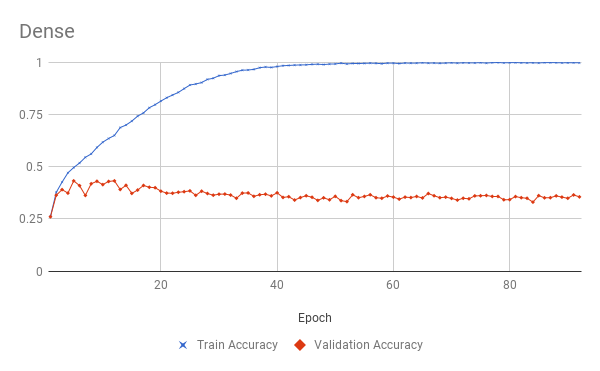
\includegraphics[scale=0.4]{dense.png}
	\caption{Acuracia para treino e validação}
	\label{fig:dense}
\end{figure}

\begin{figure}[h!]
	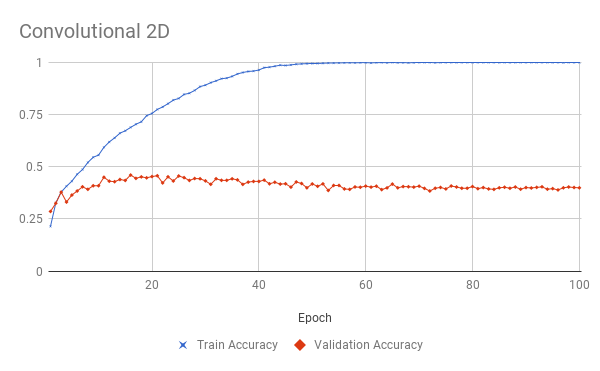
\includegraphics[scale=0.4]{conv.png}
	\caption{Acuracia para treino e validação}
	\label{fig:conv}
\end{figure}

\begin{figure}[h!]
	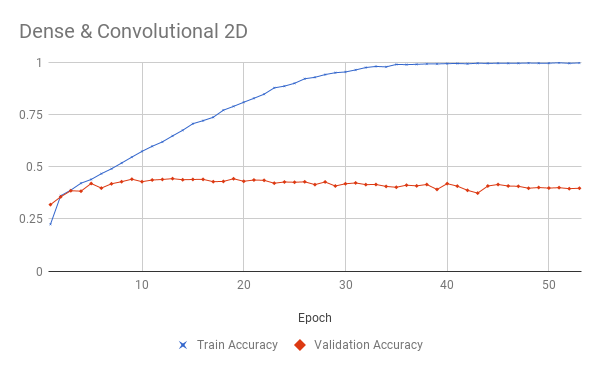
\includegraphics[scale=0.4]{dense_conv.png}
	\caption{Acuracia para treino e validação}
	\label{fig:dense_conv}
\end{figure}

\begin{figure}[h!]
	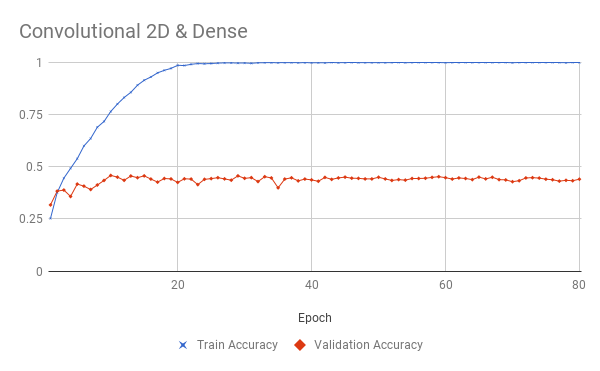
\includegraphics[scale=0.4]{conv_dense.png}
	\caption{Acuracia para treino e validação}
	\label{fig:conv_dense}
\end{figure}

Por conta da dimensão do conjunto de treino, foram utilizadas apenas 10\% das entradas. Então, o conjunto de treino foi dividido em treino e validação (utilizando uma proporção de 0.7) a fim de validar os modelos propostos. Os melhores resultados do conjunto de validação para cada modelo foram: 

\begin{itemize}
	\item Dense(512) - $0.4327$
	\item Conv2D(32, (3, 3)) - $0.4607$
	\item Dense(512) \& Conv2D(32, (3, 3)) - $0.4433$
	\item Conv2D(32, (3, 3)) \& Dense(512) - $0.4587$
\end{itemize}

Aplicando a rede neural encontrada nas melhores épocas para o modelo \textit{Conv2D(32, (3, 3))} e para o modelo \textit{Conv2D(32, (3, 3)) \& Dense(512)} utilizando o conjunto de testes, encontrou-se uma acuracia de $0.4673$ e $0.4374$, respectivamente. 

A maior acuracia encontrada pela rede \textit{Conv2D(32, (3, 3))} pode ser atribuida a quantidade reduzida de dados utilizados, visto que por ser uma rede mais simples necessita de menor número de treinos para calibrar seus valores. 

Finalmente, a fim de comparar a Ativação utilizando \textit{ReLU}, executou-se o modelo \textit{Conv2D(32, (3, 3)) \& Dense(512)} utilizando como método de ativação a Tangente Hiperbólica: $f(x) = htan(x)$. A maior acurácia encontrada para o conjunto de validação foi de $0.3320$, apontando uma vantagem para a utilização do \textit{ReLU}. 

\section{Conclusões}
Sobre as soluções propostas, aquelas que se utilizaram de processamento de imagem não trouxeram melhoras para o modelo. No entanto, a solução utilizando PCA trouxe melhoras tanto para o resultado quanto para tempo de computação do modelo, demonstrando a vantagem de usar a redução de dimensionalidade por este método.

Com relação a modelagem utilizando Redes neurais, poderia-se estudar a acuracia para um número maior de camadas, além da utilização mais estensiva de operadores convolucionais. Outra analise que pode ser feita em estudos posteriores é a utilização de Dropout, que utiliza da desativação de neurônios aleatórios de uma camada, evitando overfit e gerando redundâncias na rede neural. 

\begin{thebibliography}{00}
\bibitem{linearregression1} Montgomery, D.C., Peck, E.A. and Vining, G.G., 2015. Introduction to linear regression analysis. John Wiley \& Sons.
\bibitem{gendreau2010handbook} Gendreau, M. and Potvin, J.Y., 2010. Handbook of metaheuristics (Vol. 2). New York: Springer.
\bibitem{continousgenetics} Haupt, R.L. and Haupt, S.E., 2004. Practical genetic algorithms. John Wiley \& Sons.
\bibitem{continuousgenetics2} Djurisic, A.B., Elazar, J.M. and Rakic, A.D., 1997. Genetic algorithms for continuous optimization problems-a concept of parameter-space size adjustment. Journal of Physics A: Mathematical and General, 30(22), p.7849.
\end{thebibliography}

\end{document}
